\documentclass{article}
\usepackage[UTF8]{ctex}
\setmainfont{Calibri Light}
\usepackage{setspace}
\renewcommand{\baselinestretch}{1.2}
\usepackage{amsmath}
\usepackage{amssymb}
\usepackage{ntheorem}
\usepackage{graphicx}
\usepackage{bbm}
\usepackage{hyperref}
\hypersetup{
	colorlinks=true,
	linkcolor=blue,
	filecolor=cyan,      
	urlcolor=red,
	citecolor=green,
}
\newtheorem{theorem}{Theorem}
\newtheorem{corollary}{Corollary}
\newtheorem{lemma}{Lemma}
\newtheorem*{proof}{Proof}
\setlength{\parindent}{2em}
\author{Siheng Zhang\\zhangsiheng@cvte.com}
\title{第\textbf{\textit{1}}章\ \ \ \ 概率近似正确}
\date{\today}      
\usepackage[a4paper,left=18mm,right=18mm,top=25mm,bottom=25mm]{geometry} 

\begin{document}
\maketitle  


本章对应 \textbf{UML第2-5章},主要回答如下问题:

\begin{itemize}
\item 关于泛化误差,我们能知道什么?
\item 当我们谈论归纳偏置的时候,我们在谈论什么?
\end{itemize}

\tableofcontents
\newpage

\section{学习器形式化:输入、输出与评价}

\begin{itemize}

	\item \textbf{输入}:
	
	\begin{itemize}
	\item 实例集:实例$x \in \mathcal{X}$。
	\item 标签集:标签 $y \in \mathcal{Y}$。本章主要考虑二分类问题,即$\mathcal{Y}=\{0,1\}$。
	\item 样本集合:一个有限的序列$S=((x_1,y_1),\cdots,(x_m,y_m))$。
	\end{itemize}	 

	\item \textbf{输出}:假设(hypothesis),有时候称为分类器(classifier)、回归器(regressor) $h:\mathcal{X}\rightarrow\mathcal{Y}$.

	\item \textbf{数据生成模型}:假设实例依概率分布$\mathcal{D}$产生,并且有一个“绝对正确”的标签生成函数(至少目前我们假设如此)$f:\mathcal{X}\rightarrow\mathcal{Y}$。
	
	独立同分布(i.i.d)假设:训练样本的产生独立地来自于同一个分布。
	
	\item \textbf{泛化误差}:也称为真实误差或者真实风险。以$\mathcal{D}(A)$记观测某样例$x \in A \subset \mathcal{X}$的概率,则泛化误差为:
	
	\begin{equation}
	L_{\mathcal{D},f}(h)\overset{def}{=}\mathop{\mathbb{P}}\limits_{x\sim\mathcal{D}}[h(x)\neq f(x)]\overset{def}{=}\mathcal{D}(\{x:h(x)\neq f(x)\})
	\end{equation}
	
\end{itemize}

	\vspace{2mm}
	\begin{scriptsize}
	\begin{spacing}{1.2}
	{\sffamily
	\noindent\textit{\underline{注1.} 数据生成模型对学习器不可见。}

    \noindent\textit{\underline{注2.} 通常我们说“训练集”,但是严格来说应该说“训练序列”,因为同样的样本可以多次出现,并且一些学习算法的输出因输入顺序不同而不同。}
    
    \noindent\textit{\underline{注3.} 严格来说,$\mathcal{D}$定义在$\mathcal{X}\times\mathcal{Y}$上,但通常不严格区分。}}
	\end{spacing}
	\end{scriptsize}
	\vspace{-2mm}
	
\section{从最小经验风险到概率近似正确}

\subsection{最小经验风险(Empirical Risk Minimization,ERM) 准则可能造成过拟合}

	显然,泛化误差是不可知的。因此,我们转而最小化经验风险:

	\begin{equation}
	L_S(h)\overset{def}{=}\frac{|\left\{(x_i,y_i)\in S:h(x_i)\neq y_i \right\}|}{m}
	\end{equation}

	考虑一个“懒惰”的学习器$h$,它记下了所有的样本,当且仅当$x=x_i$时候输出$y=y_i$,其它时候都输出0。显然,它的经验风险$L_S(h)=0$,但是对于未见样本,它有一半的概率预测失败,$L_{\mathcal{D},f}(h)=1/2$。这种在训练集上表现特别好,但是泛化性能很差的现象,称为“过拟合”。这个例子蕴含着一个很重要的基本事实:
	
	\textbf{如果不对假设集加以限制,最小经验风险准则可能造成过拟合。}

\subsection{归纳偏置(inductive bias)下的最小经验风险准则}

	选取可行的假设集即反映了人对任务的先验知识,或言归纳偏置。记假设集为$\mathcal{H}$,最小经验风险准则形式化表述为:
	\begin{equation}
	h_S\in \arg\min \limits_{h\in\mathcal{H}}L_S(h)
	\end{equation}

	“理想”的情况下,假设集中包含有泛化误差为0的假设,即存在$h^*\in\mathcal{H}$使得$L_{\mathcal{D},f}(h^*) = 0$,我们称之为\textbf{可实现假设}。该条件蕴含着$L_S(h^*)=0$, $L_S(h_S)=0$,而事实上,我们更感兴趣的是$L_{\mathcal{D},f}(h_S)$。

\subsection{概率近似正确(Probably Approximately Correct,PAC)可学习性}
	\textbf{定义}:称假设集是概率近似正确可学习的,当给定大小为$m\geq m_\mathcal{H}(\epsilon,\delta)$的样本集,假设集中存在一个假设以至少$1-\delta$的置信度达到不低于$1-\epsilon$的正确率,即$P(L_{\mathcal{D},f}(h_S) < \epsilon) > 1-\delta$。
	
	\begin{theorem} 有限假设集是PAC可学习的,且样本复杂度为$m_\mathcal{H}(\epsilon,\delta)=\frac{\log(|\mathcal{H}|/\delta)}{\epsilon}$.
	\end{theorem}
	
	\begin{proof}
	记“坏”假设集为$\mathcal{H}_B$,即$\mathcal{H}_B\subset\mathcal{H}$, and $\forall h\in\mathcal{H}_B,L_{\mathcal{D},f}(h)>\epsilon$. Let $M$ be the set of 'misleading' samples, that is $M=\{S:\exists h\in \mathcal{H}_B, L_S(h)=0\}$. Note that, 
	
	\begin{equation*}
	M=\bigcup\limits_{h\in\mathcal{H}_B}\{S:L_S(h)=0\}
	\end{equation*}
	
	The goal is to bound the probability of the event $L_{\mathcal{D},f}(h_S)>\epsilon$,
	\begin{equation*}
	\begin{split}
	&\mathcal{D}^m(\{S:L_{\mathcal{D},f}(h_S)>\epsilon\})\leq\mathcal{D}^m(M) \\
	&=\mathcal{D}^m(\bigcup\limits_{h\in\mathcal{H}_B}\{S:L_S(h)=0\})         
	=\sum_{h\in\mathcal{H}_B}\prod_{i=1}^m\mathcal{D}(\{x_i:f(x_i)=h(x_i)\})  \\
	&\overset{i.i.d.}{=}\sum_{h\in\mathcal{H}_B}(1-L_{\mathcal{D},f}(h))^m   
	\leq\sum_{h\in\mathcal{H}_B}(1-\epsilon)^m\leq\sum_{h\in\mathcal{H}_B}\exp(-\epsilon m) \\
	&\leq|\mathcal{H}|\exp(-\epsilon m)
	\end{split}
	\end{equation*}

	Let $|\mathcal{H}|\exp(-\epsilon m)\leq\delta$, we can solve that $m\geq\log(|\mathcal{H}|/\delta)/\epsilon$.
	\end{proof}

\subsection{“没有免费午餐”定理}

	\begin{theorem}
	Let $A$ be any learning algorithm for the task of binary classification with respect to the 0-1 loss over a domain $\mathcal{X}$. Let $m$ be any number smaller than $\mathcal{X}/2$, representing a training set size. Then, there exists a distribution $\mathcal{D}$ over ${X}\times\{0,1\}$ such that:
	
	\begin{itemize}
	\item There exists a function $f:\mathcal{X}\rightarrow\{0,1\}$ with $L_\mathcal{D}(f)=0$.
	\item With probability of at least $1/7$ over the choice of $S\sim\mathcal{D}^m$ we have that $L_\mathcal{D}(A(S))\geq 1/8$.
	\end{itemize} 
	\end{theorem}
	
	\begin{proof}
	Let $C\subseteq\mathcal{X}$ of size $2m$. There are $T=2^{2m}$ possible functions $f_1,\cdots,f_T$ defined on $C\rightarrow\{0,1\}$. For each such function, let $\mathcal{D}_i$ be a distribution over $\mathcal{C}\times\{0,1\}$ defined as follow:
	
	\begin{equation*}
	\mathcal{D}_i(\{(x,y)\})=\left\{
	\begin{matrix} 1/|C|,& \mathrm{if}\ y=f_i(x) \\ 0,& \mathrm{otherwise} 
	\end{matrix}\right.
	\end{equation*}
	
	There are $k=(2m)^m$ possible sequences $S_1,\cdots,S_k$, each of $m$ examples from $C$. Also, we denote the sequence $\mathcal{S}_j$ labelled by the function $f_i$ as $\mathcal{S}_j^i$. If the distribution is $\mathcal{D}_i$, then the possible training sets are $S_1^i,\cdots,S_k^i$, with equal probability. Therefore,

	\begin{equation*}
	\mathop{\mathbb{E}}\limits_{S\sim\mathcal{D}_i^m}[L_{\mathcal{D}_i}(A(S))]=\frac{1}{k}\sum_{j=1}^kL_{\mathcal{D}_i}(A(S_j^i))
	\end{equation*}
	
	Using the facts that 'maximum' is larger than 'average', and that 'average' is larger than 'minimum', we have
	
	\begin{equation*}
	\max_{i\in\{1,\cdots,T\}} \frac{1}{k}\sum_{j=1}^k L_{\mathcal{D}_i}(A(S_j^i)) \geq \frac{1}{T}\sum_{i=1}^T \frac{1}{k} \sum_{j=1}^k L_{\mathcal{D}_i}(A(S_j^i)) \geq \min_{j\in\{1,\cdots,k\}}\frac{1}{T}\sum_{i=1}^T L_{\mathcal{D}_i} (A(S_j^i))
	\end{equation*}

	Next, fix some $j\in\{1,\cdots,k\}$. Denote $S_j=(x_1,\cdots,x_m)$ and let $v_1,\cdots,v_p$ be the examples in $C$ that do not appear in $S_j$. Clearly, $p\geq m$. Therefore, for every $h:C\rightarrow\{0,1\}$,
	
	\begin{equation*}
	L_{\mathcal{D}_i}(h)=\frac{1}{2m}\sum_{x\in C}\mathbbm{1}_{[h(x)\neq f_i(x)]}\geq\frac{1}{2p}\sum_{r=1}^p\mathbbm{1}_{[h(v_r)\neq f_i(v_r)]}
	\end{equation*}
and hence,

	\begin{equation*}
	\frac{1}{T}\sum_{i=1}^T L_{\mathcal{D}_i} (A(S_j^i))\geq\frac{1}{2}\min_{r\in\{1,\cdots,p\}}\frac{1}{T}\mathbbm{1}_{[A(S^i_j)(v_r)\neq f_i(v_r)]}
	\end{equation*}

	Next, fix some $r\in[p]$, We can partition all the functions $f_1,\cdots,f_T$ into $T/2$ disjoint pairs, where for a pair $(f_i,f_{i'})$ we have that $\forall c\in C,f_i(c)\neq f_{i'}(c)$ iff. $c=v_r$. Since for such a pair we must have $S_j^i=S_j^{i'}$, it follows that $\mathbbm{1}_{[A(S_j^i)(v_r)\neq f_i(v_r)]}+\mathbbm{1}_{[A(S_j^{i'})(v_r)\neq f_{i'}(v_r)]}=1$, which yields:
	
	\begin{equation*}
	\frac{1}{T}\sum_{i=1}^T\mathbbm{1}_{[A(S_j^i)(v_r)\neq f_i(v_r)]}=\frac{1}{2}
	\end{equation*}

	In conclusion, it holds that

	\begin{equation*}
	\max_{i\in\{1,\cdots,T\}}\mathop{\mathbb{E}}_{S\sim\mathcal{D}_i^m}[L_{\mathcal{D}_i}(A(S))]\geq 1/4
	\end{equation*}

	This means that for every algorithm, there exists $f,\mathcal{D}$, such that $L_\mathcal{D}(f)=0$ and $\mathop{\mathbb{E}}\limits_{S\sim\mathcal{D}^m}[L_\mathcal{D}(A(S))]\geq 1/4$.

	\textit{(following is part of UML Ex5.1)} For a random variable $\theta\in[0,1]$ such that $\mathbb{E}(\theta)\geq 1/4$, we have:
	
	\begin{equation*}
	p\left(\theta\geq\frac{1}{8}\right)=\int_\frac{1}{8}^1 p(\theta) \mathrm{d}\theta \geq\int_\frac{1}{8}^1 \theta p(\theta) \mathrm{d}\theta=\mathbb{E}(\theta)-\int_0^\frac{1}{8}\theta p(\theta)\mathrm{d}\theta \geq\mathbb{E}(\theta)-\frac{1}{8}\int_0^\frac{1}{8} p(\theta)\mathrm{d}\theta = \frac{1}{4} - \frac{1}{8}\left( 1-\int^1_\frac{1}{8}p(\theta) \mathrm{d}\theta \right)
	\end{equation*}
which leads to $p(\theta\geq 1/8)\geq 1/7$.
	\end{proof}

	\textbf{NFL theorem tells the necessity of inductive bias.} Philosophically, if someone can explain every phenomenon, his explanations are worthless.
	
\section{不可知情况下的PAC(Agnostic PAC, A-PAC)可学习性}
	\subsection{在可实现假设之外}
	In practical, the 'true' labelling function may not exist, and the labels may not be fully determined by the features on hand. Then Agnostic PAC learnability is defined as: training on $m\geq m_\mathcal{H}(\epsilon,\delta)$ samples, there exists an algorithm with \textbf{confidence} at least $1-\delta$ to achieve that:
	
	\begin{equation*}
	L_\mathcal{D}(h)\leq\min\limits_{h'\in\mathcal{H}}L_\mathcal{D}(h')+\epsilon
	\end{equation*}
in which $L_\mathcal{D}(h)\overset{def}{=}\mathop{\mathbb{P}}\limits_{(x,y)\sim\mathcal{D}}[h(x)\neq y]\overset{def}{=}\mathcal{D}(\{x:h(x)\neq y\})$.

	\subsection{在二分类之外}

	仅需修改对单个样例损失的刻画,A-PAC可学习性仍表述为:
	
	\begin{equation}
	\mathcal{D}(h)=\mathop{\mathbb{E}}\limits_{x\sim\mathcal{D}}[l(h,z)]
	\end{equation}
in which $l(\cdot)$ is 0-1 loss for multi-class classification and square loss for regression. 

	\subsection{A-PAC可学习假设集的样本复杂度}
	
	\textbf{Definition} ($\epsilon$-representative): A training set $S$ is called $\epsilon$-representative (w.r.t. domain $Z$, hypothesis set $\mathcal{H}$, loss function $l$, and distribution $\mathcal{D}$) if $\forall h\in\mathcal{H},|L_S(h)-L_\mathcal{D}(h)|\leq\epsilon$.
	
	\begin{lemma}
	Assume that a training set $S$ is $\epsilon/2$-representative. Then, any $h_S\in\arg\min_{h\in\mathcal{H}}L_S(h)$ satisfies
	\begin{equation}
	L_\mathcal{D}(h_S) \leq L_S(h)+\epsilon
	\end{equation}
	\end{lemma}
	
	\begin{proof}
	for every $h\in\mathcal{H}$,
	
	\begin{equation*}
	L_\mathcal{D}(h_S) \leq L_S(h_S)+\frac{\epsilon}{2}
	\leq L_S(h)+\frac{\epsilon}{2} \leq L_\mathcal{D}(h)+\frac{\epsilon}{2}+\frac{\epsilon}{2}
	\leq L_\mathcal{D}(h)+\epsilon
	\end{equation*}	 
	\end{proof}
	
	The lemma states that the ERM learning rule is guaranteed to return a good hypothesis for any $\epsilon/2$-representative sample set. It implies that to ensure that the ERM rule is an agnostic PAC learner, it suffices to show that with probability of at least $1-\delta$ over the random choice of a training set, it will be an $\epsilon$-representative training set. The following definition measures how many examples we need to ensure this condition.
	
\noindent\textbf{Definition} (Uniform Convergence): We say that a hypothesis class $\mathcal{H}$ has the uniform convergence property if there exists a function $m^{UC}_\mathcal{H}:(0,1)^2\rightarrow \mathbb{N}$ such that for every $\epsilon,\delta \in (0, 1)$ and for every probability distribution $\mathcal{D}$ over $Z$, if $S$ is a sample set of size $m\geq m^{UC}_\mathcal{H}(\epsilon, \delta)$ examples drawn i.i.d. according to $\mathcal{D}$, then, with probability of at least $1-\delta$, $S$ is $\epsilon$-representative.

	\begin{corollary}
	If a class $\mathcal{H}$ has the uniform convergence property with a function $m^{UC}_\mathcal{H}$ then the class is agnostic PAC learnable with the sample complexity $m_\mathcal{H}(\epsilon,\delta)\leq m^{UC}_\mathcal{H}(\epsilon/2,\delta)$, and the ERM$_\mathcal{H}$ paradigm is a successful agnostic PAC learner for $\mathcal{H}$.
	\end{corollary}
	
	\begin{lemma}
	(Hoeffding's Inequality) Let $\theta_1,\cdots,\theta_m$ be a sequence of i.i.d. random variables and assume that $\forall i, \mathbb{E}[\theta_i]=\mu$ and $P[a\leq\theta_i\leq b]=1$. Then, for any $\epsilon>0$,
	\begin{equation*}
	P\left[\left| \frac{1}{m}\sum_{i=1}^m\theta_i - \mu \right| >\epsilon \right] \leq 2 \exp \left( \frac{-2m\epsilon^2 }{(b-a)^2} \right)
	\end{equation*}
	\end{lemma}

	\begin{theorem}
	\textbf{Agnostic PAC sample complexity} Assume that the range of the loss function is $[a,b]$, then a finite hypothesis set $\mathcal{H}$ enjoys the agnostic PAC learnability with sample complexity 
	
	\begin{equation}
	m_\mathcal{H}(\epsilon,\delta)\leq m^{UC}_\mathcal{H}(\epsilon/2,\delta)\leq\left\lceil\frac{2\log(2|\mathcal{H}|/\delta)(b-a)^2}{\epsilon^2}\right\rceil
	\end{equation}
	
	\begin{proof}
	Fix some $\epsilon,\delta$, we need to find a sample size $m$ that guarantees that: For any $\mathcal{D}$, with probability of at least $1-\delta$ of the choice of $S=(z_1,\cdots,z_m)$ sampled i.i.d. from $\mathcal{D}$, such that
	\begin{equation*}
	\mathcal{D}^m(\{S:\exists h\in\mathcal{H}, |L_S(h)-L_\mathcal{D}(h)|>\epsilon\}) < \delta
	\end{equation*}
	Since
	\begin{equation*}
	\{S:\exists h\in\mathcal{H}, |L_S(h)-L_\mathcal{D}(h)|>\epsilon\} = \cup_{h\in\mathcal{H}}\{S:|L_S(h)-L_\mathcal{D}(h)|>\epsilon\}
	\end{equation*}
the left side can be bounded by
	\begin{equation*}
	\mathcal{D}^m(\{S:\exists h\in\mathcal{H}, |L_S(h)-L_\mathcal{D}(h)|>\epsilon\}) \leq \sum_{h\in\mathcal{H}} \mathcal{D}^m(\{S:|L_S(h)-L_\mathcal{D}(h)|>\epsilon\})
	\end{equation*}
	Recall that $L_S(h)=\frac{1}{m}\sum_{i=1}^m l(h,z_i)$ and $L_\mathcal{D}(h)=\mathbb{E}_{z\sim\mathcal{D}}[l(h,z)]$. Since each $z_i$ is sampled i.i.d. from $\mathcal{D}$, by the linearity of expectation, $\mathbb{E}(L_S(h))=\frac{1}{m}\sum_{i=1}^m \mathbb{E}(l(h,z_i))=L_\mathcal{D}(h)$. Hence, the quantity $|L_\mathcal{D}(h)-L_S(h)|$ is the deviation of the random variable $L_S(h)$ from its expectation. We therefore need to show that the measure of $L_S(h)$ is concentrated around its expected value. Using the Hoeffding's Inequality directly leads to the following:
	\begin{equation*}
	\mathcal{D}^m(\{S:|L_S(h)-L_\mathcal{D}(h)|>\epsilon\}) \leq 2 \exp \left( \frac{-2m\epsilon^2 }{(b-a)^2} \right)
	\end{equation*}
	Combining the equations above,
	\begin{equation*}
	\mathcal{D}^m(\{S:\exists h\in\mathcal{H}, |L_S(h)-L_\mathcal{D}(h)|>\epsilon\}) \leq \sum_{h\in\mathcal{H}} 2 \exp \left( \frac{-2m\epsilon^2 }{(b-a)^2} \right) = 2|\mathcal{H}|\exp \left( \frac{-2m\epsilon^2 }{(b-a)^2} \right)
	\end{equation*}
	Choose $m\geq\frac{2\log(2|\mathcal{H}|/\delta)(b-a)^2}{\epsilon^2}$, then the left-side is bounded by $\delta$.
	\end{proof}	
	\end{theorem}

\section{误差分解}

	\begin{equation}
	\begin{split}
	L_\mathcal{D}(h_S) &= \epsilon_{\mathrm{app}}+\epsilon_{\mathrm{est}} \\
	\epsilon_{\mathrm{app}} &= \min\limits_{h\in\mathcal{H}}L_\mathcal{D}(h) \\
	\epsilon_{\mathrm{est}} &= L_\mathcal{D}(h_S)-\epsilon_{\mathrm{app}}
	\end{split}
	\end{equation}		

	\begin{itemize}
	\item \textbf{逼近误差} measures how much risk we have because we restrict ourselves to a specific class, namely, how much inductive bias we have. The approximation error does not depend on the sample size and is determined by the hypothesis class chosen. Enlarging the hypothesis class can decrease the approximation error.
	\item \textbf{拟合误差} measures the empirical risk (i.e., training error), which is only an estimate of the true risk. The quality of this estimation depends on the training set size (decreases with it) and on the size, or complexity, of the hypothesis class (logarithmically increases with it).
	\end{itemize}

\section{总结}

	\vspace{2mm}
	\begin{scriptsize}
	\begin{spacing}{1.2}
	{\sffamily
	\noindent\textit{\underline{注.} 在本系列笔记的整理过程中,这一小节的出现意味着,这章枯燥且乏味,但这章的偏理论的内容是不需要记住的,因为这些推导所指向的下述结论是非常浅显的。小结最后还会写到,这章的内容将如何与其它章节前后关联,以使读者明白其在整个机器学习理论中所处的地位。如果某些章没有这一小节,那么说明该章节的内容浅显易懂,不需要这一小节。)
	}}
	\end{spacing}
	\end{scriptsize}
	\vspace{2mm}

	至此,在PAC学习理论框架下,我们有了如下重要结论:
\begin{enumerate}
\item No universal learner;
\item Inductive bias is neccessary to avoid overfitting;
\item Sample complexity is function about hypothesis set, confidence level and error, interestingly, it is nothing to do with the dimension of feature space;
\item Inductive bias controls the balance of approximation error and estimation error.
\end{enumerate}

	We have reached the fundamental question in learning theory: \textbf{Over which hypothesis classes, ERM learning will not result in overfitting (or, PAC learnable)?} Currently, we just confirm the PAC learnability for finite classes. In the next chapter, the most important part in learning theory, VC-dimension, will gives a more precise answer.


\section{练习与答案}

\begin{itemize}
\item[Ex1] (UML Ex2.2) Let $\mathcal{H}$ be a class of binary classifiers over a domain $\mathcal{X}$. Let $\mathcal{D}$ be an unknown distribution over $\mathcal{X}$, and let $f$ be the target hypothesis in $\mathcal{H}$. Fix some $h\in\mathcal{H}$, show that the expected value of $L_S(h)$ over the choice of $S$ equals $L_{\mathcal{D},f}(h)$, namely,

\begin{equation*}
\mathop\mathbb{E}\limits_{S\sim\mathcal{D}^m}[L_S(h)]=L_{\mathcal{D},f}(h)
\end{equation*}

\item[] \textbf{Solution}: By the linearity of expectation,
\begin{equation*}
\begin{split}
\mathop\mathbb{E}\limits_{S\sim\mathcal{D}^m}[L_S(h)] 
&= \mathop\mathbb{E}\limits_{S\sim\mathcal{D}^m}[\frac{1}{m}\sum_{i=1}^m \mathbbm{1}_{[h(x_i)\neq f(x_i)]}] \\
&= \frac{1}{m}\sum_{i=1}^m \mathop\mathbb{E}\limits_{x_i \sim\mathcal{D}^m}[\mathbbm{1}_{[h(x_i)\neq f(x_i)]}] \\
&= \frac{1}{m} \cdot m \cdot L_{\mathcal{D},f}(h) = L_{\mathcal{D},f}(h)
\end{split}
\end{equation*}

\item[Ex2] (UML Ex2.3) \textbf{Axis Aligned rectangles}: An axis aligned rectangle classifier in the plane is a classifier that assigns the value 1 to a point if and only if it is inside a certain rectangle. Formally, given real numbers $a_1\leq b_1,a_2\leq b_2$, define the classifier $h(a_1,b_1,a_2,b_2)$ by:

	\begin{equation*}
	h(a_1,b_1,a_2,b_2)(x_1, x_2) = \left\{\begin{matrix}
	1,& \mathrm{if}\ a_1 \leq x_1 \leq b1\ \mathrm{and}\  a_2 \leq x_2 \leq b_2 \\
	0,& \mathrm{otherwise}
	\end{matrix}\right.
	\end{equation*}

	The class of all axis aligned rectangles in the plane is defined as:
	
	\begin{equation*}
	\mathcal{H}^2_{\mathrm{rec}}=\{h_{(a_1,b_1,a_2,b_2)}:a_1\leq b_1,\ \mathrm{and}\ a_2\leq b_2\}
	\end{equation*}
Note that this is an infinite size hypothesis class. Throughout this exercise we rely on the realizability assumption.

	\begin{itemize}
	\item[2.1] Let $A$ be the algorithm that returns the smallest rectangle enclosing all positive examples in the training set. Show that $A$ is an ERM.
	\item[2.2] Show that if $A$ receives a training set of size $\geq 4\frac{\log(4/\delta)}{\epsilon}$, then, with probability of at least $1-\delta$ it returns a hypothesis with error of at most $\epsilon$.
	
	\textit{Hint: Fix some distribution $\mathcal{D}$ over $\mathcal{X}$, let $R^*=R(a^*_1,b^*_1,a^*_2,b^*_2)$ be the rectangle that generates the labels, and let $f$ be the corresponding hypothesis. Let $a_1\geq a^*_1$ be a number such that the probability mass (with respect to $\mathcal{D}$) of the rectangle $R_1=R(a^*_1,a_1,a^*_2,b^*_2)$ is exactly $\epsilon/4$. Similarly, let $b_1,a_2,b_2$ be numbers such that the probability masses of the rectangles $R_2=R(b_1,b^*_1,a^*_2,b^*_2)$, $R_3=R(a^*_1,b^*_1,a^*_2,a_2)$, $R_4=R(a^*_1,b^*_1,b_2,b^*_2)$ are all $\epsilon/4$. Let $R(S)$ be the rectangle returned by $A$. See illustration in the following figure.}
	
	\begin{figure}[!htbp]
	\center
	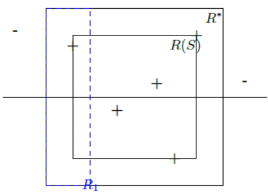
\includegraphics[scale=.8]{1.png}
	\end{figure}
	
	\begin{itemize}
	\item Show that $R(S)\subseteq R^*$.
	\item Show that if $S$ contains (positive) examples in all of the rectangles $R_1,R_2,R_3,R_4$, then the hypothesis returned by $A$ has error of at most $\epsilon$.
	\item For each $i\in\{1,\cdots,4\}$, upper bound the probability that $S$ does not contain an example from $R_i$.
	\item Use the union bound to conclude the argument.
	\end{itemize}
	 
	\item[2.3] Repeat the previous question for the class of axis aligned rectangles in $\mathbb{R}^d$.
		
	\item[2.4] Show that the runtime of applying the algorithm $A$ mentioned earlier is polynomial in $d, 1/\epsilon$, and in $\log(1/\delta)$.
	\end{itemize}

	\item[] \textbf{Solution}
	
	\begin{itemize}
	\item[2.1] In realizable setup, since the tightest rectangle enclosing all positive example is returned, all positive and negative instances are correctly classified.
	\item[2.2] By definition, algorithm A returns the tightest rectangle, so $R(S)\subseteq R^*$. 
	\end{itemize}

\item[Ex3] (UML Ex3.2) Let $\mathcal{X}$ be a discrete domain, and let $\mathcal{H}_{\text{Singleton}}=\{h_z:z\in\mathcal{X}\}\cup\{h^-\}$, where for each $z\in\mathcal{X}$, $h_z$ is the function defined by $h_z(x)=1$ if $x=z$ and $h_z(x)=0$ if $x\neq z$. $h^-$ is simply the all-negative hypothesis, namely, $\forall x\in\mathcal{X},h^-(x)=0$. The realizability assumption here implies that the true hypothesis $f$ labels negatively all examples in the domain, perhaps except one.

	\begin{itemize}
	\item[3.1] Describe an algorithm that implements the ERM rule for learning $\mathcal{H}_{\text{Singleton}}$ in the realizable setup.
	\item[3.2] Show that $\mathcal{H}_{\text{Singleton}}$ is PAC learnable. Provide an upper bound on the sample complexity.
	\end{itemize} 

	\item[] \textbf{Solution}:
	\begin{itemize}
	\item[3.1] Traverse $z\in\mathcal{X}$ then output $h_z$ or $h^-$.
	\item[3.2] If for any $i\in[1,\cdots,m]$, $h_{x_i}$ is the true hypothesis, the algorithm can find it in the realizable setup. Otherwise, the algorithm outputs $h^-$, which can be either true or false (i.e., the target $z^*$ is not in the training set). Note that in the second case, the algorithm only makes a single error when generalize to all cases, and hence $p(z^*)\geq\epsilon$ (otherwise, it is meaningless),
	
	\begin{equation*}
	\mathbb{P}(L_{\mathcal{D},f}(h_S)>\epsilon)\leq(1-p(z^*))^m\leq(1-\epsilon)^m\leq\exp(-\epsilon m)\leq\delta
	\end{equation*}

which leads to
	\begin{equation*}
	m_\mathcal{H}(\epsilon,\delta)\leq\left\lceil\frac{\log(1/\delta)}{\epsilon}\right\rceil
	\end{equation*}
	

\item[Ex4] (UML Ex3.3) Let $\mathcal{X}=\mathbb{R}^2$, $\mathcal{Y}=\{0,1\}$, and let $\mathcal{H}$ be the class of concentric circles in the plane, that is, $\mathcal{H}=\{h_r:r\in\mathbb{R}_+\}$, where $h_r(x)=\mathbbm{1}_{[\| x\|\leq r]}$. Prove that $\mathcal{H}$ is PAC learnable (assume realizability), and its sample complexity is bounded by:

	\begin{equation*}
	m_\mathcal{H}(\epsilon,\delta)\leq\left\lceil\frac{\log(1/\delta)}{\epsilon}\right\rceil
	\end{equation*}
	
	\item[] \textbf{Solution} Denote the probability of $x$ such that $r\leq\|x\|_2\leq r^*$ is $\epsilon$, then:
	\begin{equation*}
	P(L_\mathcal{D}(h_r(S))\geq\epsilon) \leq (1-\epsilon)^m \leq e^(-m\epsilon)
	\end{equation*}
Bound it by confidence $\delta$ leads to the conclusion.
	
\item[Ex5] (UML Ex3.4) In this question, we study the hypothesis class of Boolean conjunctions defined as follows. The instance space is $\mathcal{X} = \{0, 1\}^d$ and the label set is $\mathcal{Y} = \{0, 1\}$. A literal over the variables $x_1, \cdots, x_d$ is a simple Boolean function that takes the form $f(\mathbf{x}) = x_i$, for some $i\in [d]$, or $f(\mathbf{x}) = 1-x_i$ for some $i\in [d]$. We use the notation $\overline{x}_i$ as a shorthand for $1-x_i$. A conjunction is any product of literals. In Boolean logic, the product is denoted using the $\wedge$ sign. For example, the function $h(\mathbf{x}) = x_1 \cdot (1 - x_2)$ is written as $x_1 \wedge \overline{x}_2$.

	We consider the hypothesis class of all conjunctions of literals over the $d$ variables. The empty conjunction is interpreted as the all-positive hypothesis (namely, the function that returns $h(\mathbf{x}) = 1$ for all $\mathbf{x}$). The conjunction $x_1 \wedge \tilde{x}_1$ (and similarly any conjunction involving a literal and its negation) is allowed and interpreted as the all-negative hypothesis (namely, the conjunction that returns $h(\mathbf{x}) = 0$ for all $\mathbf{x}$). We assume realizability: Namely, we assume that there exists a Boolean conjunction that generates the labels. Thus, each example $(x, y)\in\mathcal{X}\times\mathcal{Y}$ consists of an assignment to the $d$ Boolean variables $x_1, \cdots, x_d$, and its truth value (0 for false and 1 for true). For instance, let $d = 3$ and suppose that the true conjunction is $x_1 \wedge \overline{x}_2$. Then, the training set $S$ might contain the following instances:
	\begin{equation*}
	((1, 1, 1), 0), ((1, 0, 1), 1), ((0, 1, 0), 0), ((1, 0, 0), 1)
	\end{equation*}

	Prove that the hypothesis class of all conjunctions over $d$ variables is PAC learnable and bound its sample complexity. Propose an algorithm that implements the ERM rule, whose runtime is polynomial in $d\cdot m$.

\item[] \textbf{Solution}: $\mathcal{H}$ is finite, and hence is PAC learnable. Besides the all-negative conjunction, each hypothesis is determined by deciding for each variable $x_i$ with 3 possible choices ( $x_i$,  $\overline{x}_i$ or none). Thus,  $\mathcal{H}=3^d+1$, and 

	\begin{equation*}
	m_\mathcal{H}(\epsilon, \delta) \leq \left\lceil \frac{d\log 3 + \log(1/\delta)}{\epsilon} \right\rceil
	\end{equation*}
	
	Below is the learning algorithm. Start from $h=x_1\wedge\overline{x}_1\wedge\cdots\wedge x_d\wedge\overline{x}_d$, which is always negative. The algorithm does nothing when feed a negative example, and remove $x_1$ or $\overline{x}_1$ when feed a positive example. With realizability assumption, it can labels all training examples correctly and hence is an ERM. Since the algorithm takes linear time (in terms of the dimension $d$) to process each example, the running time is bounded by $O(m\times d)$.
	
\item[Ex6] (UML Ex3.7) The Bayes optimal predictor: Show that for every probability distribution $\mathcal{D}$, the Bayes optimal predictor $f_\mathcal{D}$ is optimal, in the sense that for every classifier $g$ from $X$ to $\{0, 1\}$, $L_\mathcal{D}(f_{\mathcal{D}}) \leq L_\mathcal{D}(g)$.

\item[] \textbf{Solution}: The Bayes predictor labels a sample $x$ according to

	\begin{equation*}
	f_\mathcal{D}(x) = \left\{
	\begin{matrix} 0,& \mathrm{if}\ \mathcal{D}((x,0))\geq \mathcal{D}((x,1)) \\ 1,& \mathrm{otherwise} 
	\end{matrix}\right.
	\end{equation*}
	
	When it labels a sample to be class 0, it holds that $\mathcal{D}((x,0))\geq \mathcal{D}((x,1))$. If the true label function also makes such a decision, then Bayes predictor makes no error. Otherwise, $f(x)=1$, but its probability is no more than 1/2. Any other classifier that labels $x$ to be class 1 will suffer a risk no less than 1/2. Hence, in total, Bayes predictor is the optimal.

\item[Ex7] (UML Ex3.9) Consider a variant of the PAC model in which there are two example oracles: one that generates positive examples and one that generates negative examples, both according to the underlying distribution $\mathcal{D}$ on $\mathcal{X}$. Formally, given a target function $f: \mathcal{X}\rightarrow\{0,1\}$, let $\mathcal{D}^+$ be the distribution over $\mathcal{X}^+ = \{x\in\mathcal{X}: f(x)= 1\}$ defined by $\mathcal{D}^+(A) = \mathcal{D}(A)/\mathcal{D}(\mathcal{X}^+)$, for every $A\in\mathcal{X}^+$. Similarly, $\mathcal{D}^-$ is the distribution over $\mathcal{X}^-$ induced by $\mathcal{D}$. 
	
	The definition of PAC learnability in the two-oracle model is the same as the standard definition of PAC learnability except that here the learner has access to $m_\mathcal{H}^+(\epsilon, \delta)$  i.i.d. examples from $\mathcal{D}^+$ and $m^-(\epsilon, \delta)$ i.i.d. examples from $\mathcal{D}^-$. The learner's goal is to output $h$ s.t. with probability at least $1-\delta$ (over the choice of the two training sets, and possibly over the nondeterministic decisions made by the learning algorithm), both $L(\mathcal{D}^+, f)(h)\leq\epsilon$ and $L(\mathcal{D}^-, f)(h)\leq\epsilon$.
	\begin{itemize}
	\item[7.1] Show that if $\mathcal{H}$ is PAC learnable in the standard one-oracle model, then $H$ is PAC learnable in the two-oracle model.
	\item[7.2] Define $h^+$ to be the always-plus hypothesis and $h^-$ to be the always minus hypothesis. Assume that $h^+, h^-\in \mathcal{H}$. Show that if $\mathcal{H}$ is PAC learnable in the two-oracle model, then $\mathcal{H}$ is PAC learnable in the standard one-oracle model.
	\end{itemize}
	
	\item[] \textbf{Solution}:
	\begin{itemize}
	\item[7.1] Drawing points from the negative and positive oracles with equal provability is equivalent to obtaining i.i.d. examples from a distribution $\mathcal{D}'$ which gives equal probability to positive and negative examples. If we let an algorithm to access to a training set which is drawn i.i.d. according to the $\mathcal{D}'$ with size $m_\mathcal{H}(\epsilon/2, \delta)$, then with probability at least $1-\delta$, it returns $h$ with:
	\begin{equation*}
	\begin{split}
	& \epsilon/2 \geq L_{(\mathcal{D}',f)}(h) = \mathop{\mathbb{P}}\limits_{x\sim\mathcal{D}'}[h(x)\neq f(x)] \\
	& = \mathop{\mathbb{P}}\limits_{x\sim\mathcal{D}'}[f(x)=1, h(x)=0] + \mathop{\mathbb{P}}\limits_{x\sim\mathcal{D}'}[f(x)=0, h(x)=1] \\
	& = \mathop{\mathbb{P}}\limits_{x\sim\mathcal{D}'}[f(x)=1] \cdot \mathop{\mathbb{P}}\limits_{x\sim\mathcal{D}^+}[h(x)=0] + \mathop{\mathbb{P}}\limits_{x\sim\mathcal{D}'}[f(x)=0] \cdot \mathop{\mathbb{P}}\limits_{x\sim\mathcal{D}^-}[h(x)=1] \\
	& = \frac{1}{2}L_{(\mathcal{D}^+,f)}(h) + \frac{1}{2}L_{(\mathcal{D}^-,f)}(h)
	\end{split} 
	\end{equation*}
which implies $L_{(\mathcal{D}^+,f)}(h)\leq\epsilon$ and $L_{(\mathcal{D}^-,f)}(h)\leq\epsilon$.
	\item[7.2] 
	\end{itemize}
	
\item[Ex8] (UML Ex5.3) Prove that if $|\mathcal{X}|\geq km$ for a positive integer $k\geq 2$, then we can replace the lower bound in the No-Free-Lunch theorem. Namely, for the task of binary classification, there exists a distribution $\mathcal{D}\sim\mathcal{X}\times\{0,1\}$ such that:

	\begin{itemize}
	\item[8.1] There exists a function $f:\mathcal{X}\rightarrow\{0,1\}$ with $L_\mathcal{D}(f)=0$.
	\item[8.2] $\mathbb{E}_{S\sim\mathcal{D}^m}[L_\mathcal{D}(A(S))]\geq\frac{1}{2}-\frac{1}{2k}$.
	\end{itemize}

\item[] \textbf{Solution}:
	Only the second proposition should be proved. Similar with the proof in above, 
	\begin{equation*}
	L_{\mathcal{D}_i}(h)=\frac{1}{km}\sum_{x\in C}\mathbbm{1}_{[h(x)\neq f_i(x)]}\geq\frac{1}{km}\sum_{r=1}^p\mathbbm{1}_{[h(v_r)\neq f_i(v_r)]}\geq\frac{k-1}{pk}\sum_{r=1}^p\mathbbm{1}_{[h(v_r)\neq f_i(v_r)]}
	\end{equation*}
 
And similarity,

	\begin{equation*}
	\frac{1}{T}\sum_{i=1}^T L_{\mathcal{D}_i} (A(S_j^i))\geq\frac{k-1}{k}\min_{r\in\{1,\cdots,p\}}\frac{1}{T}\mathbbm{1}_{[A(S^i_j)(v_r)\neq f_i(v_r)]}
	\end{equation*}
	
	So the final bound is $1/2-1/2k$.
\end{itemize} 

\end{itemize}

\end{document}